\chapter{Results}

This chapter will go through the whole process of making, training and testing the \gls{gnn} step by step, from first iterations of the very simple model to more fine tuned models and other methods that were tested. Reasoning and explanations for the choices and changes made during the process will also be given along the way. Finally, best results that were achieved will be presented. 

All the experiments have been done on the same machine with: 11th Gen Intel(R) Core(TM) i7-11700K 3.60GHz 8-core CPU, 16 GB RAM and NVIDIA RTX 3080Ti graphics card.

\section{Progress}
\subsection{Simple line graph model}

First step was to try the simplest model with most of the hyperparameters set to default and train it on a smaller scale. First model had 2 layers and 64 neurons each. Initially due to majority of nodes being not included in the matching, the model learned to set all nodes to be dropped and still get a rather high accuracy score. This was resolved by adding class weights as a training parameter. Class weights tell the model how important each class is. By assigning the nodes that go into matching a value of 0.9 and the ones that do not 0.1. The problem seemed to be resolved.
 
Trained on a 1000 MNIST graphs model resulted on average with 55\% of optimal weight possible. This was an expected result considering the limitation, but it at least showed that model is gaining some knowledge compared to untrained model as well as a solution that randomly picks edges, where both resulted in 50-51\% of optimal. 

A model that barely beats random solution is not very usefull. Poor performance for now is mainly due to the very limited training, but before adding more data and prolonging training, we can experiments with the parameters of the network to see if they make any impact.

\subsection{Model improvements and data augmentation}

At this stage model seemed to at slowly improve and learn, but before trying to train it on the whole dataset there were still other techniques and parameters worth testing. Each of the techniques was tested separately. 

It would make sense to start with the depth and width of the network. After trying to add up to 6 layers, it showed that more than 3 layers did not have any significant effect. Note: layers tell how many generations of neighbors is used for representation of a node. Increasing breadth did help, but impact got smaller as the breadth got wider. It would also impact running time so it was decided to have the model with 2 layers and 640 nodes at each layer (except input/output layers). Results were, however still rather low at  58\%.

Next step was to adjust optimizer parameters: learning rate and weight decay. Too high learing rates resulted in too unstable training with information loss jumping too much, which indicated that model made too big adjustments after each training iteration. Too low learning rate did not give enough progress and made training proccess too slow. Value of 0.001 worked well as a middle ground.

Weight decay is another hyperparameter that can help with training the model. It can help to keep weight values relatively small and decrease chances of the model memorizing the answers, also called overfitting. However only negative effect were noticed even when training with larger datasets.

Adding skip connections to the architecture adds alternative way for the information to flow through the network. Skip connections help the model to reuse information from previous layers. No significant effect was noticed with only tenths of a percent improvement in performance, possibly due to the network having too few layers. Still, it was decided to keep the skip connections since they did not harm in anyway and could be helpfull later.

Augmenting node features was another technique that was tested. The graphs were preproccessed  Trying each additional feature separately to see it they have any benefits by themselves, then adding them one by one. Finally using all at once since they can mostly be calculated simultaneously and all have at least some positive effect:

\begin{figure}[H]
    \centering
    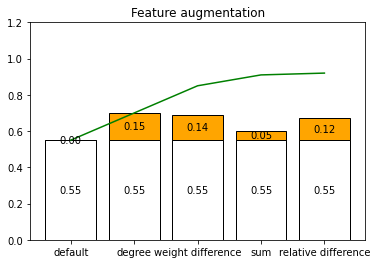
\includegraphics[scale=1.0]{figures/FeatureAugmentationLine}
    \caption{MNIST trained model. Average performance on 100 MNIST graphs}
    \label{Feature Augmentation Effect}
\end{figure}

With fine tuning og the models hyperparameters and architecture, and augmenting node features having the most effect on the performance, results were moving closer to reasonable. At this point full training set can be used to see proper results. The results were relatively promising, but further testing showed that unfortunately line graph transformation on large and dense enough graphs turned out to expode in size and take to much time to proccess. Therefore another architecture was considered.
 
\section{Edge prediction model}

Instead of turning edges to nodes model can give predictions on the node pairs directly. With this approach there is less preprocessing needed, but the model now needs to have an extra layer for edge prediction as described in \hyperref[sec:architecture]{Architecture section}.
After training both edge classification model and line graph model on the 55000 MNIST graphs following results were recorded: 101\% for edge classification and 103\% for line graph.

MNIST trained Model's performance on unseen MNIST graphs
\begin{figure}[H]
    \centering
    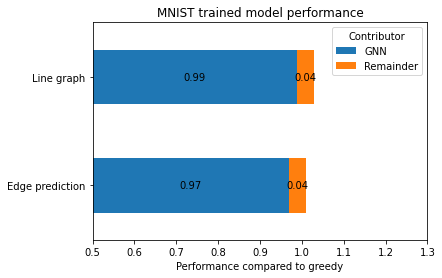
\includegraphics[scale=1.0]{figures/FinalPerformanceMNIST}
    \caption{MNIST performance comparison}
    \label{Model performance on MNIST}
\end{figure}

Edge classification showed a little bit worse results on average than the line graph. In theory it can be due to line graph containing more structural information in it compared to original. Regardless of the slightly worse result edge classification approach was still favourable due to time consumption of the line graph convertion. The results themselves were rather promising, both models manage to beat the greedy algorithm even when the greedy result is close to the optimal. However, there is still another probelm, time. Due to the small size of MNIST graphs finding optimal solution using Blossom algorithm takes less time than using this \gls{gnn} model, because of the overehad computations needed for the neural network, but the model should be able to catch up timewise when given larger graphs. There is still the question of whether training on small graphs can help with larger graphs. The next step is to test the current model on a different graph - Cage10 from SuiteSparse. Cage10 is a graph with 11000 ndoes and 100 000 edges and the model produces following results: 

\begin{figure}[H]
    \centering
    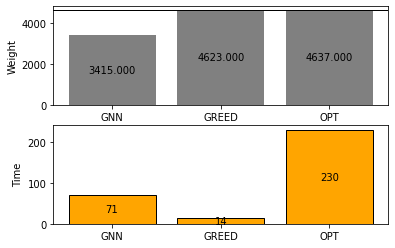
\includegraphics[scale=1.0]{figures/MNISTtrainCAGE10}
    \caption{MNIST trained model performance on cage10 graph}
    \label{model performance}
\end{figure}

As seen on the figure above \gls{gnn} manages to beat the optimal solver in term of time, but it is noticeably worse in terms of total weight. Poor performance can be caused by the current training dataset. One of the main interests was to see if the \gls{gnn} can be used on graphs larger than the ones it was trained on. It could be that model fails to learn what is needed for larger graphs. Another reason could be that MNIST graphs have similar structure without enough variety to cover other graph types. One of course cannot include all the possible graphs in the training set, but the more data and variety model gets during training the better. Therefore another dataset was tried for training. A custom dataset consisting of randomly picked graphs from the SuiteSparse database. This custom dataset consists of 1000+ graphs with varying sizes and structures, between 100 and 10000 nodes.

Training the same model on the new dataset showed that model struggled to learn the patterns. The flat information loss during training indicated that model had hard time to learn the more diverse collection of graphs. Adding additional layer to the classifier module of the model helped with stagnating learning curve. Adding even more layers did not give any noticeable difference like adding the first layer did. A slighly deeper than the previous model gave the following results on the new dataset:

\begin{figure}[H]
    \centering
    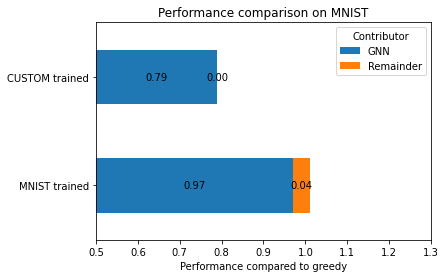
\includegraphics[scale=1.0]{figures/MNISTvsCUSTOMonMNIST}
    \caption{MNIST vs CUSTOM dataset training model performance on MNIST graphs}
    \label{models performance comparison}
\end{figure}

As partially expected model trained using custom dataset performed noticeably worse than the model trained on exclusively MNIST graphs. The custom dataset had both less graphs and larger graphs, than the ones in the MNIST dataset. This could be improved by adding some MNIST graphs to the custom dataset, but the main goal now is to see if the new dataset helps to get better performance on larger graphs. 

\begin{figure}[H]
    \centering
    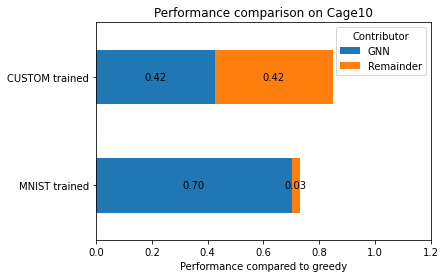
\includegraphics[scale=1.0]{figures/MNSITvsCUSTOMonCage10}
    \caption{MNIST vs CUSTOM dataset training model performance on cage10}
    \label{models performance comparison}
\end{figure}

\begin{figure}[H]
    \centering
    \includegraphics[scale=1.0]{figures/CUSTOMtrainCAGE10}
    \caption{CUSTOM trained model performance on cage10 graph}
    \label{model performance}
\end{figure}

The custom trained model does perform better in this case, however it is not neccesarily the models accuracy itself that is the reason of improvement. The model seems to be rather indecisive on which nodes to match and half of the graph at the end is left unmatched opposed to the MNIST trained model matching almost the whole graph itself. This does however spark an idea that one might use the model to only match the most important nodes with highest probabilities and leave the rest to the greedy algorithm to achieve better results. 

Results are still unsatisfying and there is a couple other ideas left to try: adjusting matching threshold for the model and applying reduction.

\subsection{Reduction}

Reduction rules are used in algorithms to cut down the size of the graphs by removing the easily recognizable parts of the graphs. Ideally the neural network should be able to pick up such, but it is still worth testing to see if there is any positive effect as well as see if model manages to grasp such rules by itself. The reduction rule itself is rather simple. If two connected nodes have an edge with a weight larger than the weight of the largest outgoing edge of each node there is no raeson to not pick it, since it is impossible to get a larger weight form these nodes.

\begin{comment}
\begin{algorithmic}[H]
\KwData{$graph G$}
\ForAll{$edge e$}
	\If{$e.weight > weight sum of largest remaining edge weights of the nodes$}
		\STATE $Pick the edge$\;
	\EndIf
\EndFor
\end{algorithmic}
\end{comment}

\begin{figure}[H]
    \centering
    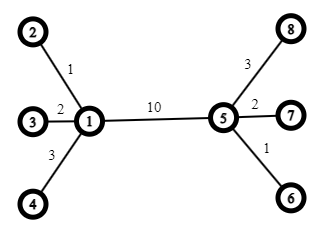
\includegraphics[scale=1.0]{figures/ReductionExample}
    \caption{Reduction example}
    \label{Reduction example}
\end{figure}

A couple different graphs were used to test if the reduction helps and whether the model could find reducible nodes on its own. On some cases there were graphs that had 0 reducible edges, but in other cases such edges made around 5\% of the total amount. The model however did not seem to pick any of those edges and adding reduction as a preprocessing step did improve the results by a small margin. Since the reduction is based on the largest edges of the nodes it would make sense to add these node features to the model. 
New model was trained with 2 additional node features: 1st largest weight, 2nd largest weight for each node.
Adding such features could in theory have helped the model to find reducible nodes, but after training the new model with the new node features the result did not improve.

\subsection{Matching threshold}

Adjusting the threshold for picking the edges was another thing to test as the previous results suggested. The model was initialy set to only consider edges that it predicted to have a larger than 50\% chance of being part of the solution. This mathing treshold can be adjusted to for example only pick the edges with 90\% probabilty, this can help focus the model on the edges that have large impact on the total result, but would be otherwise ignored by a greedy algorithm. Additionaly it can be worth testing removal of edges with low probabilties to see if model can find edges that if picked inhibit the overall result.

\begin{figure}[H]
    \centering
    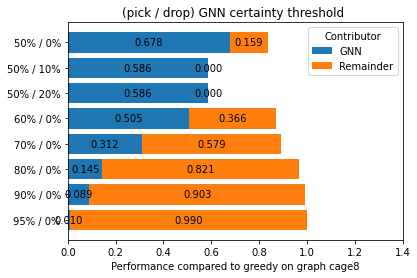
\includegraphics[scale=1.0]{figures/ThresholdDemo}
    \caption{Model threshold test on cage8 graph}
    \label{Model threshold test}
\end{figure}

The higher matching threshold does seem to improve the performance, but not enough to beat the greedy algorithm and most likely the increase is caused by the larger remainder due to fewer edges being above the treshold. Adding the drop threshold did not seem to work that well either. The model seems to assign very low scores to a lot of edges which results in worse results and no remainder to compensate. The reason for that is probably the weight class hyperparameter used during training which makes the model to care less for correctly finding nodes that should be ignored. The better approach could be to train model specifically to find high value edges.

\section{Final results}

With time remaining and ideas for further improvements starting to end, the final best model was tested on increasingly larger graphs from different sources. The final parameters of the model were:

\begin{enumerate}
\item Learning rate = 0.001
\item Epochs = 100
\item Mini-batch size = 1
\item Network depth and width = 4 layers, 640 neurons each
\item Class weights = 0.1 and 0.9 for dropped and picked edges respectively
\item Weight decay = 0
\item Match threshold = 70\%
\item Added pre computed node features
	\begin{itemize}
	\item Degree - how many neighbours a node has.
	\item Sums of the weights. 	
	\item Weights sum relative to the neighbours.
	\item Weights sum difference compared to the neighbours.
	\end{itemize}
\end{enumerate}

\begin{figure}[H]
    \centering
    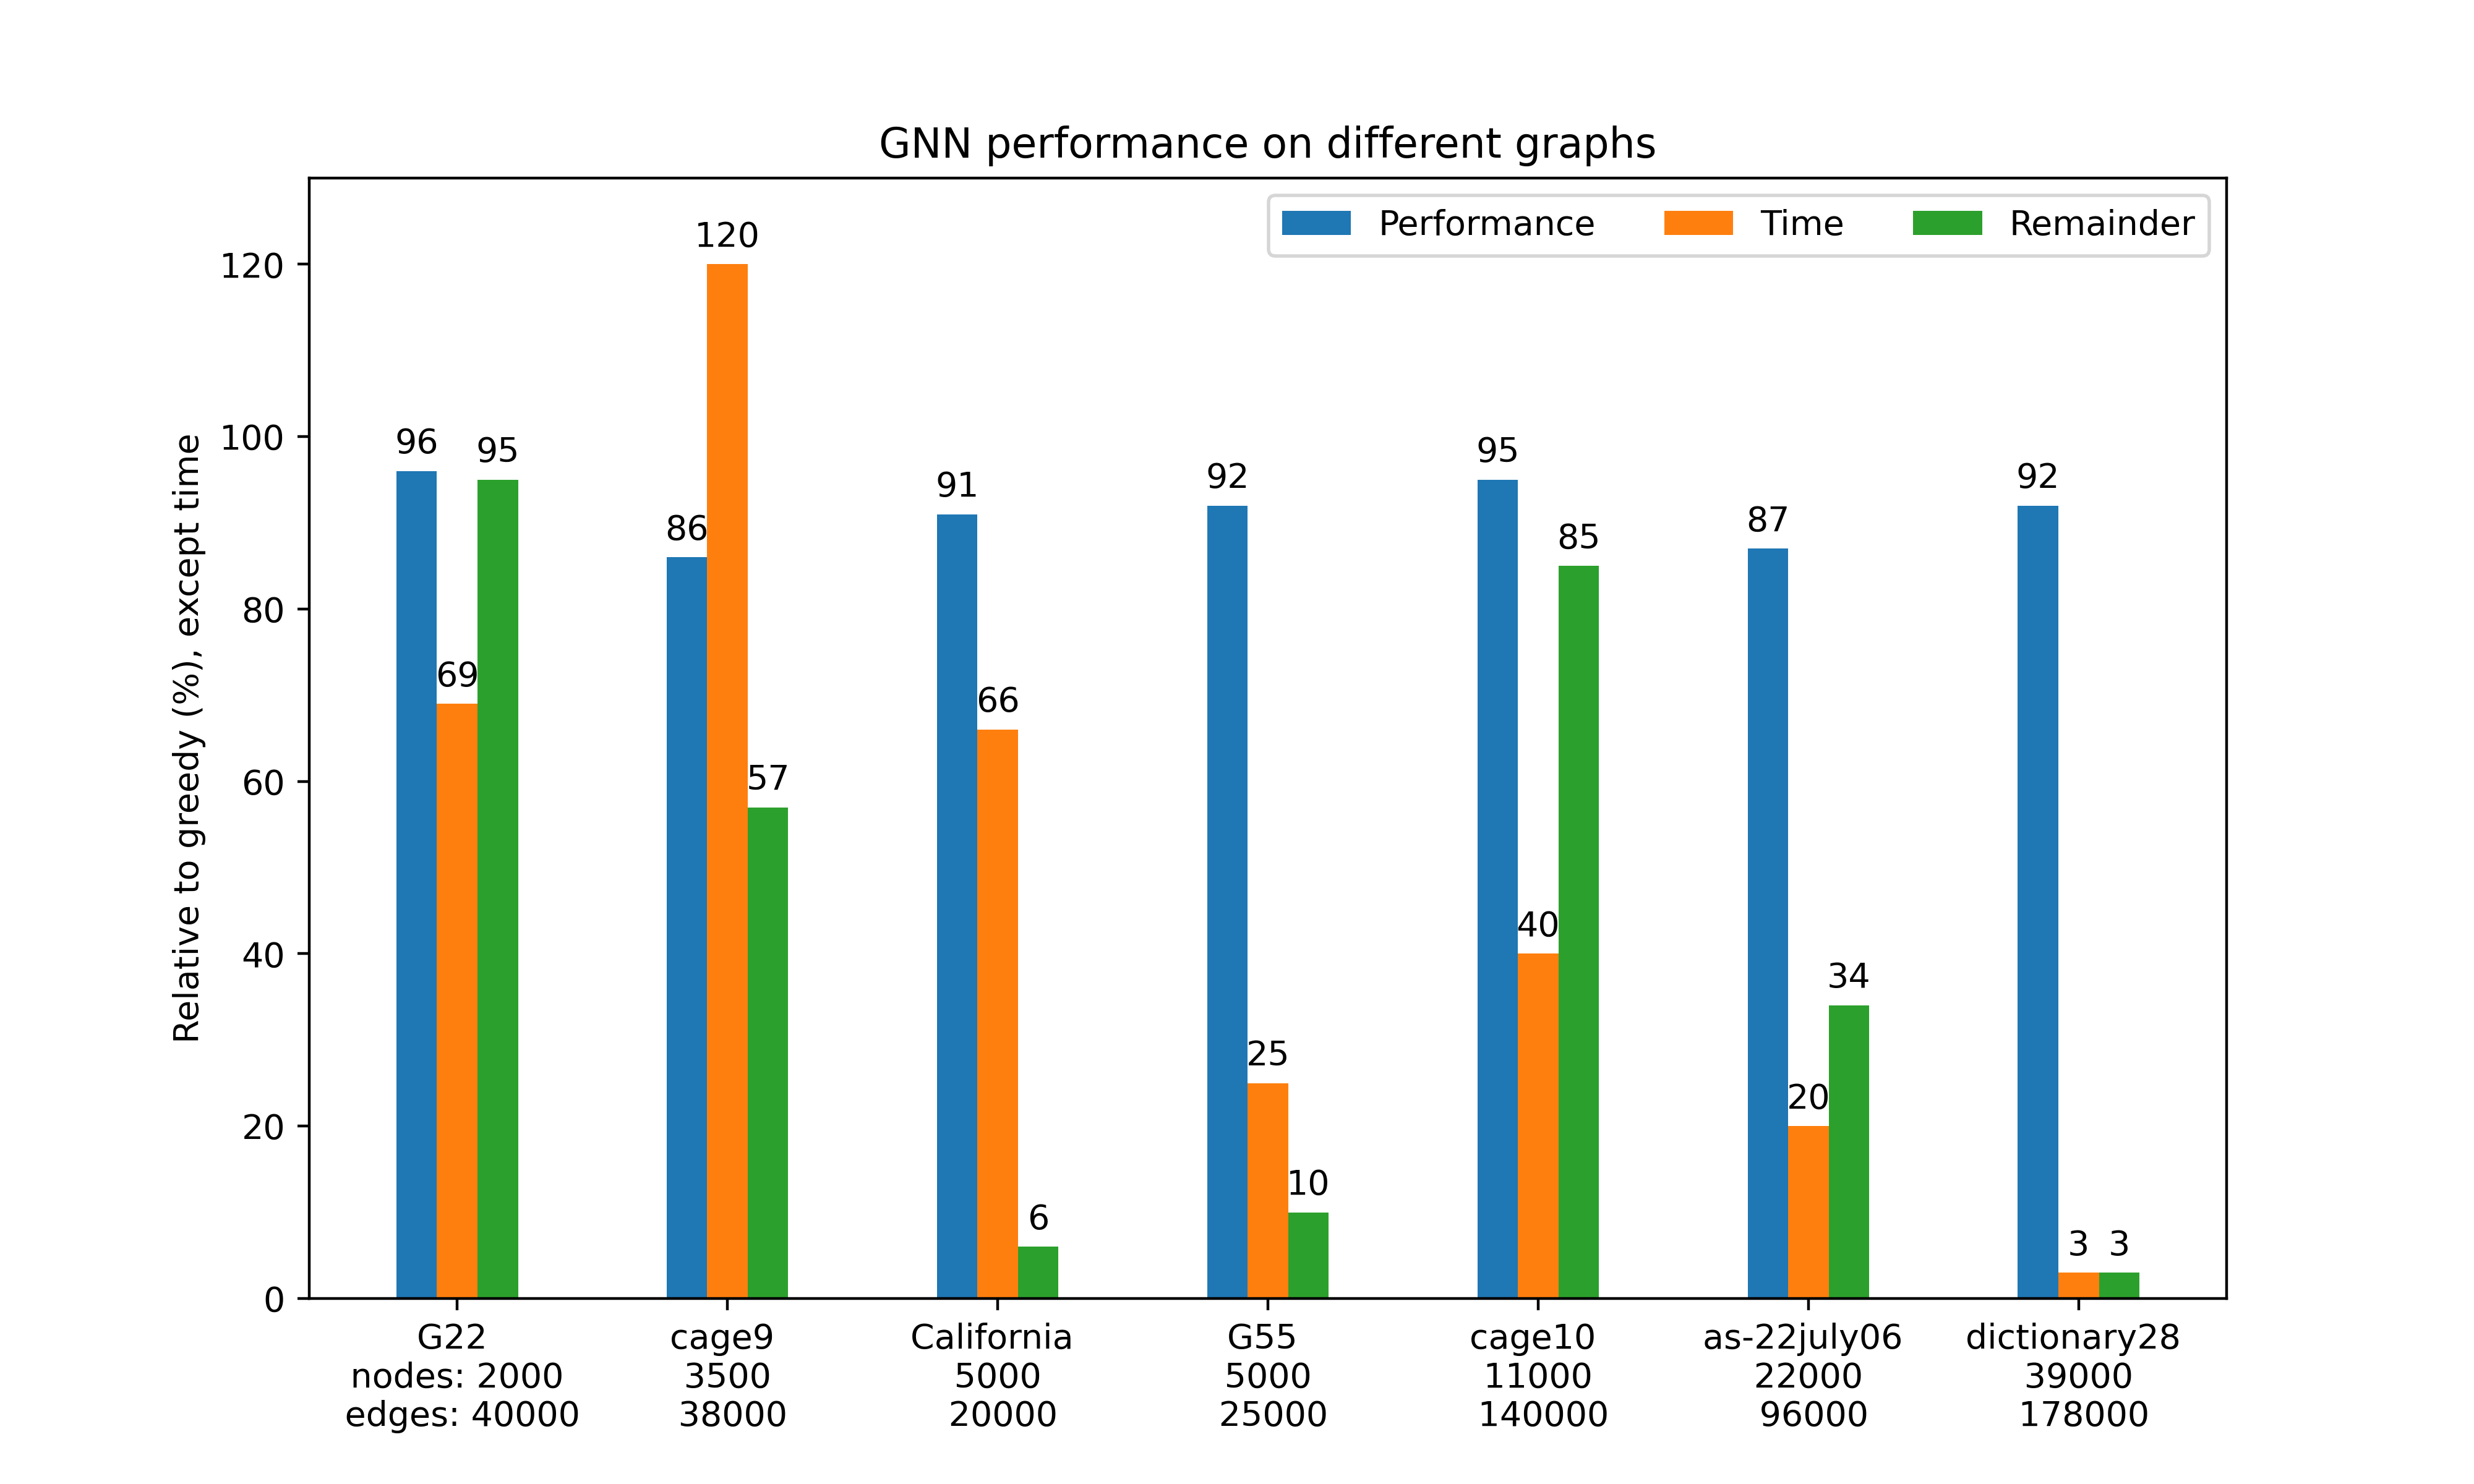
\includegraphics[scale=0.8]{figures/FINALResults}
    \caption{Final model performance}
    \label{final model performance}
\end{figure}

Lets summarize the end results based on the main criterias.
\begin{itemize}
\item Performance: The total weight the model's output seems to be rather stable at around 90\% of what greedy algorithm produces regardless of the size of the graph. It seems to be rather challenging for the model to beat the greedy approach when in most cases in makes up around 90-95\% of the total weight possible.
\item Running time: An exception in the sense that the time is shown in comparison to the time it takes to find the optimal solution. Reason for that is the fact that the model is always slower than the greedy algorithm. As expected the benefit of using the \gls{gnn} can be seen as the size of the graphs increases. Smaller graphs take more time for the model to solve due to the overhead computations needed, but as the graphs grow the running time can get as small as 3\% of the Blossom algorithm.
\item Remainder: In some cases the reason for the total weight being close to the greedy is the fact that the remainder makes up a large part of the graph, but it is not a consistent trend and neither does it depend on the size of the graph. There are cases with equally good results where the remainder is below 10\% of the total graph. The fact that some graphs leave such a big remainder indicates that the training dataset is not good enough and the model is not trained well enough to handle such graphs.
\end{itemize}

\subsection{Weakness of greedy algorithm}

On average greedy algorithm seems to show really good results, but in theory it is not hard to make a graph that abuses the greedy approach and results in poor performance. Example of a graph that \gls{gnn} model should be able to beat:

\begin{figure}[H]
    \centering
    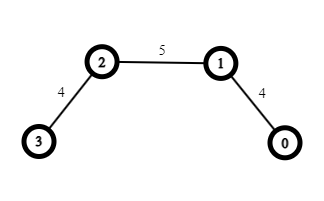
\includegraphics[scale=1.0]{figures/GoodCase}
    \caption{Good case for GNN}
    \label{Good case for GNN}
\end{figure}

In this very simple case the greedy algorithm will result in total weight = 5. Yet the \gls{gnn} does manage to get the optimal weight = 8. This ofcourse does not neccesarily prove anything, but shows that there might be use cases for the model. There are more realistic graphs that the model also manages to solve better. 1138bus graph from SuitSparse is one of the examples where \gls{gnn} outperforms greedy by 15\%. Additionaly, given that the runing times of greedy and \gls{gnn} combined are still lower than running time of finding the optimal solution, one may even run both and choose the better result.

